\documentclass[conference]{IEEEtran}
\usepackage{amsmath,amssymb,graphicx,booktabs,url}
\newcommand{\missing}{\textbf{N/A: experiment required}}
\graphicspath{{../results/audited/figures/}}
\begin{document}
\title{V-TRACE+: Auditing Diagnosis-Aware Hallucination Detection,\\Repair Routing, and Verification for Vision-Language Models}
\author{\IEEEauthorblockN{Swati, Vaishnavi, Vikas M L, Lakshmi Shree M S}
\IEEEauthorblockA{Department of Computer Science and Engineering\\
Cambridge Institute of Technology, KR Puram, Bengaluru--560036, India\\
swati.23cse@cambridge.edu.in, vaishnavi.23cse@cambridge.edu.in\\
vikas.23cse@cambridge.edu.in, lakshmi.cse@cambridge.edu.in}}
\maketitle

\begin{abstract}
Hallucination detection is useful only if subsequent intervention improves
grounding without discarding correct answers. We audit V-TRACE+, a CPU-friendly
visual-compatibility prototype with optional remote vision-language inference,
and formulate a reproducible diagnosis--route--repair--verify protocol.
Reanalysis of archived POPE-derived predictions identifies 67 unique
image--claim pairs from 34 images. On the common 32-claim, 18-image cohort,
CLIP-grid obtains AUROC 0.955 and F1 0.955, while whole-image SigLIP obtains
0.932 and 0.930. These are exploratory compatibility results, not standard
generated-answer POPE results. After deduplication, each of two selective
prediction runs correctly decides 10 of 17 claims; a confidence-only baseline
matches this performance at identical coverage. A standalone diagnosis
classifier achieves 0.980 accuracy on synthetic holdout data, but only
0.301--0.319 after a controlled count-pattern shift. We report these negative
findings and release label-isolated evaluation, recorded API smoke traces,
image-cluster statistics, and a preservation-aware repair protocol. Superiority
of diagnosis-aware repair routing remains an untested hypothesis.
\end{abstract}
\begin{IEEEkeywords}
vision-language models, hallucination, selective prediction, repair verification,
reproducibility, evaluation audit
\end{IEEEkeywords}

\section{Introduction}
Vision-language models (VLMs) can mention absent objects, miscount instances,
misattribute properties, or assert unsupported relations. A description can
contain supported and unsupported facts simultaneously. Decomposing responses
into claims permits localized inspection, but neither a similarity score nor
a fluent explanation establishes factual correctness or a latent failure cause.
Moreover, reducing hallucination by abstaining or shortening an answer may
reduce its usefulness. We therefore ask: \emph{can predicted error-type routing
improve verified answer correctness and preservation over uniform or
detection-only intervention at matched cost and coverage?}

This paper is an audit and research-protocol report, not a claim of a completed
new benchmark or state-of-the-art mitigation. Its contributions are: (i) a
traceable reanalysis correcting cohort and selective-baseline comparisons;
(ii) a controlled failure of a synthetic diagnosis classifier under feature
shift; and (iii) an executable, label-isolated closed-loop protocol with
explicit rejected repairs and measured call traces. Claims of improved
natural-data repair utility are reserved for independently annotated tests.

\section{Related Work and Novelty Boundary}
CHAIR evaluates object hallucination in captions against visual labels
\cite{chair}; POPE uses object-presence questions with different negative
sampling schemes \cite{pope}. AMBER covers existence, attributes and relations
\cite{amber}; HallusionBench probes visual illusion and language hallucination
\cite{hallusion}. MMHal-Bench originates in factually augmented RLHF
\cite{rlhf}, while M-HalDetect supplies fine-grained annotations and preference
optimization \cite{mhal}.

Atomic fact extraction and verification are established by FaithScore
\cite{faith}. Woodpecker already combines concept extraction, visual validation
and hallucination correction \cite{wood}. VCD contrasts original/distorted
visual inputs \cite{vcd}; OPERA modifies decoding using over-trust penalties
\cite{opera}; HALC uses adaptive focal grounding \cite{halc}. M3ID amplifies
visual information against language priors \cite{m3id}. Therefore these
components are not individually novel here.

Selective classification \cite{selective}, probability calibration
\cite{calibration}, sampling consistency \cite{selfcheck} and cost-aware model
routing \cite{route} also precede this project. Particularly, VISOR explicitly
couples visual/prior diagnosis with routed remediation \cite{visor}; this
invalidates a broad ``first diagnosis-to-routing'' claim. Recent evaluation
work cautions that conservative generation may improve hallucination scores
while harming informativeness \cite{safe}. The unresolved contribution is
\emph{preservation-aware, cost-matched intervention selection}, not the mere
presence of a taxonomy or router.

\section{Problem Formulation and Taxonomy}
Inputs are image $I$, question $q$, and original VLM response $a$. A decomposer
produces claims $c_i$ and exact source spans where possible. Independent gold
annotations record claim truth, required answer information, error content,
and corrected answers. Gold is never supplied to detection, routing, repair,
or candidate verification.

We separate observable \emph{error content}---object, attribute, counting,
spatial, relation, OCR, reasoning, knowledge, unsupported inference---from
unobserved \emph{mechanisms}. Legacy M0--M4 labels mix these concepts: the live
rule system uses no fault, prior override, perception/count, uncertainty and
binding; the offline classifier uses grounded, object, count, conflicting
evidence and spatial/relation. These labels are hypotheses and engineering
categories, not established causal ground truth. Unknown/ambiguous evidence
must remain representable rather than forced into a confident mechanism.

\section{Architecture and Evidence Attribution}
\begin{figure}[t]
\centering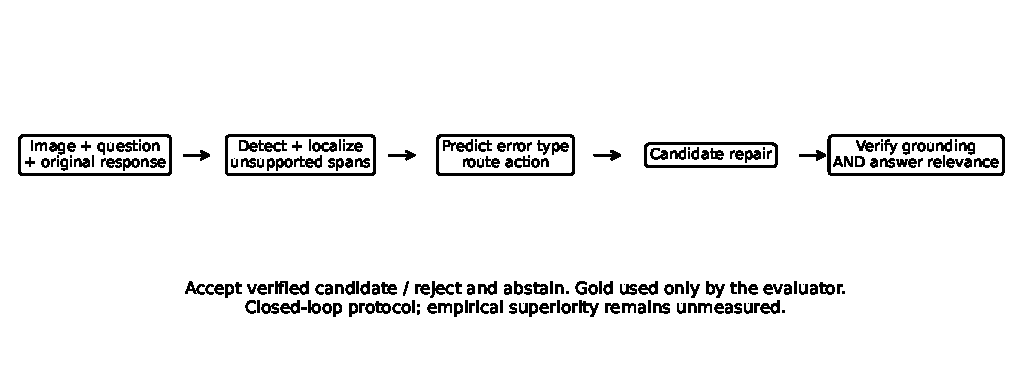
\includegraphics[width=\columnwidth]{architecture_audited.pdf}
\caption{Audited closed-loop protocol. Prediction inputs exclude gold. An
accepted candidate must pass both visual-support and question-relevance checks.
This figure describes an implementation/protocol, not measured superiority.}
\label{fig:architecture}
\end{figure}
The legacy Studio supports user text or Gemini description/decomposition.
Its local fallback splits sentences and does not guarantee atomic facts.
Frozen CLIP/SigLIP encoders compare claims to the full image and grid crops.
OWL-ViT supplies open-vocabulary proposals for optional counting. Gemini
supplies descriptions, lexical sampling-consistency inputs and YES/NO
cross-checks. Local execution is CPU-compatible; remote API execution is not
CPU-only total compute. Qwen is optional and not required by the final API path.

For raw cosine $s$, the legacy normalized support is
\begin{equation}
u(s)=\operatorname{clip}\left((s-\ell)/(h-\ell),0,1\right),\qquad
r=\sum_j w_j(1-u_j).
\end{equation}
In the evaluated Studio configuration, v1 averages region and whole-image
risks. v2 changes weights under confidence/evidence discrepancy and detector
disagreement, but confidence/probe/counterfactual channels are disabled in the
CPU text path. Optional OWL and Gemini results are auxiliary evidence, not
validated jointly calibrated probabilities. Legacy negation inversion and v3
pairwise margins are heuristic; the latter falls back to absolute scores for
ties. Different cosine windows invalidate cross-model score-gap comparisons.

The new research runner requires typed atomic claims, predicted error type,
risk, verdict and reasons. Exact source matching yields spans; absent exact
matches are null rather than fuzzy ``proof.'' Visual evidence from a model
must retain its source and uncertainty. A crop chosen by similarity is not
an independently annotated object box.

\section{Routing, Repair, and Verification}
\subsection{Preservation-aware acceptance}
The implemented extension records original facts with stable IDs, source spans
and observed evidence states. Facts judged supported are protected; this does
not make them ground truth. A text-only audit aligns every original fact to the
candidate as preserved, contradicted, omitted or uncertain, requiring exact
candidate quotes for positive alignment claims. Missing IDs, duplicate IDs,
unverifiable quotes or incomplete candidate-fact extraction reject the audit.
Separately, all extracted candidate facts require visual support, and the
candidate must answer the original question. Acceptance additionally requires
retention of all protected facts and resolution of previously refuted facts.
Removal of a refuted fact is recorded separately from correcting an answer.

Predicted-type and fixed-repair arms use the same preservation gate. A
gate-disabled ablation collects the same audit calls but ignores preservation
for acceptance, isolating the policy from its additional compute. Contract
tests show that supported-fact deletion is rejected despite a whole-answer
judge's approval. Actual API smoke traces exercise a mixed, author-edited
development response; they have no independent accuracy labels. Consequently,
natural-data preservation improvement, routing benefit and scientific novelty
remain \missing. False-positive original support and mistaken semantic
alignments can still block useful repairs or approve harmful ones.

Actions include visual, attribute, count, spatial/relation, OCR and reasoning
rechecks, with abstention for unsupported external knowledge. In the current
research backend these are explicitly named \emph{prompt adaptations}; they
are not implementations of VCD, an OCR specialist, or a validated causal
intervention. One bounded candidate repair is generated. A separate verifier
call receives $I,q,a'$ without the detector's desired verdict and checks
visual support and whether $a'$ answers $q$. Both checks must be positive to
accept; rejection retains the original in the trace and abstains. Different
Gemini versions are not assumed statistically independent.

Controlled arms use the same inputs: original output, detector-only, uniform
reinspection/correction, detect-then-fixed, surface-type routing, seeded random
routing, no diagnosis, no final verifier and full loop. Authentic published
baselines and outcome-trained routing are \missing. Missing model responses
or malformed outputs cause recorded failures, not synthetic success.

\section{Training Audit}
The existing offline diagnosis model is sklearn
\texttt{GradientBoostingClassifier}: 150 estimators, learning rate 0.05,
maximum depth 3, random state 42, multiclass log loss. It uses six numeric
features: similarity, regional evidence, detected count, claimed count,
sampling consistency and a synthetic ``Gemini confidence'' field. Generator
seed 0 produces 200 rows per class; a stratified split yields 800 training and
200 holdout rows. There is no neural optimizer, batch size or epoch schedule.
No natural image-derived diagnosis training is established, and the model is
not connected to the Studio.

A new CPU training command requires explicit image-group train/calibration
partitions and rejects test rows. Its natural-data result is \missing.
Existing Qwen LoRA code has overlapping validation, unmasked prompt labels
and incomplete multimodal collation; the launcher is quarantined. There is no
validated LoRA/SFT/DPO checkpoint or training-time/memory result.

\section{Experimental Setup}
We reanalyze four saved POPE-derived runs, deduplicating identical image/claim
pairs and checking conflicting labels/scores. The union has 67 claims from 34
images. Different methods cover different subsets; the common comparison uses
32 claims from 18 images (22 absent-object positives, 10 present-object
negatives). Claims are parsed from benchmark questions, not original VLM
answers. This task is \emph{object-phrase compatibility}, not the official
generated-answer POPE evaluation. Previously inspected images and thresholds
are development-exposed and cannot be retroactively labeled clean test data.

Analysis uses Python 3.11.7, NumPy 1.26.4, sklearn 1.6.1 and SciPy 1.17.1;
the complete environment and source/data hashes accompany the artifacts.
AUROC, average precision, F1 at 0.5, precision, recall, Brier and ten-bin ECE
are computed from saved scores. Uncertainty uses 1,000 image-cluster bootstrap
resamples (seed 42); paired randomization swaps complete image blocks. These
small-sample exploratory tests are not preregistered confirmatory evidence.

\section{Results and Statistical Analysis}
\begin{table}[t]
\caption{Matched exploratory cohort: 32 claims, 18 images. All methods use the
same cases. No full repair-system result is represented by these encoder rows.}
\centering\resizebox{\columnwidth}{!}{\begin{tabular}{lrrrrrr}
\toprule
Method & Acc. & Prec. & Rec. & F1 & AUROC & ECE \\
\midrule
siglip-whole & 0.906 & 0.952 & 0.909 & 0.930 & 0.932 & 0.259 \\
clipB32-grid & 0.938 & 0.955 & 0.955 & 0.955 & 0.955 & 0.297 \\
siglip-grid & 0.656 & 1.000 & 0.500 & 0.667 & 0.941 & 0.349 \\
\bottomrule
\end{tabular}
}
\label{tab:main}
\end{table}
Table~\ref{tab:main} reports the matched comparison. CLIP-grid minus whole
SigLIP accuracy is 0.03125, with image-cluster percentile interval
$[0,0.0968]$ and paired cluster randomization $p=1.0$. Thus superiority is not
established. SigLIP-grid's lower F1 illustrates that high ranking AUROC need
not yield reliable thresholded decisions. Per-method availability cohorts
remain in the audit but are not compared as matched ablations.

After deduplication, each archived v3 run contains 17 claims from ten images.
v3 decides ten correctly and abstains on seven (coverage $10/17$). A simple
baseline selecting the same number of most-extreme SigLIP scores also decides
ten correctly. The previously advertised selective gain over forced answers
does not demonstrate a benefit over matched-coverage selection.

\begin{figure}[t]
\centering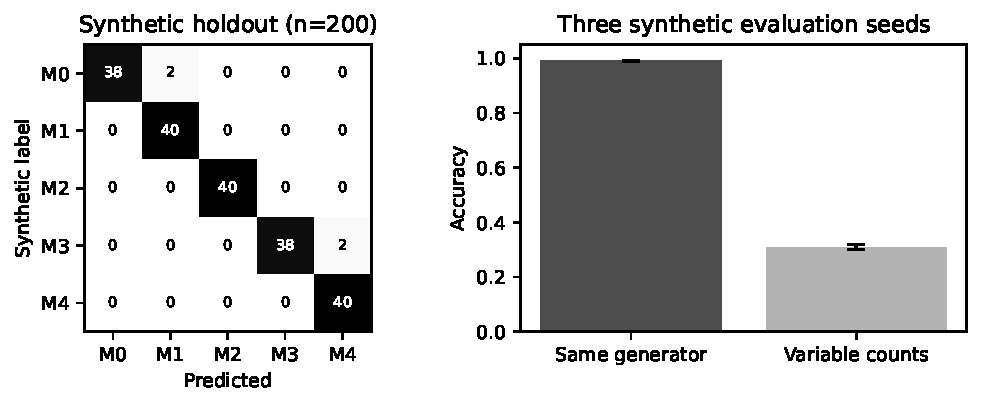
\includegraphics[width=\columnwidth]{diagnosis_shift.pdf}
\caption{Synthetic diagnosis stress test. The original GBM recovers its
generator's labels but fails when fixed count patterns change while
equality/mismatch relationships are retained. Not natural-data accuracy.}
\label{fig:shift}
\end{figure}
The synthetic GBM reproduces holdout accuracy 0.980. On new seeds 11, 12 and
13 of the same generator, accuracy is 0.989, 0.990 and 0.992. Replacing fixed
counts with variable counts preserving equality/mismatch relationships reduces
accuracy to 0.308, 0.319 and 0.301 (Fig.~\ref{fig:shift}). This controlled
negative result suggests generator-specific shortcuts rather than a robust
diagnosis model. It does not quantify performance on natural hallucinations.

\section{Calibration and Selective Prediction}
\begin{figure}[t]
\centering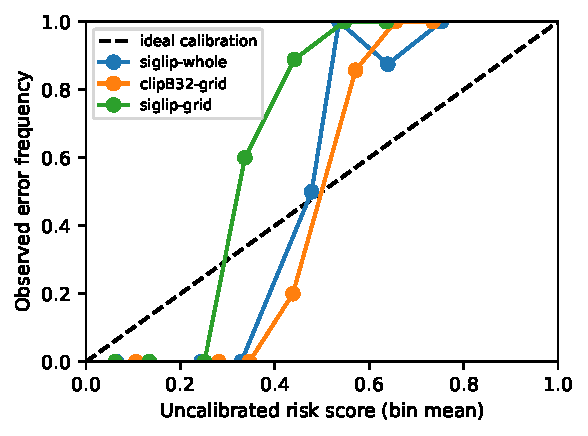
\includegraphics[width=.49\columnwidth]{calibration_raw.pdf}\hfill
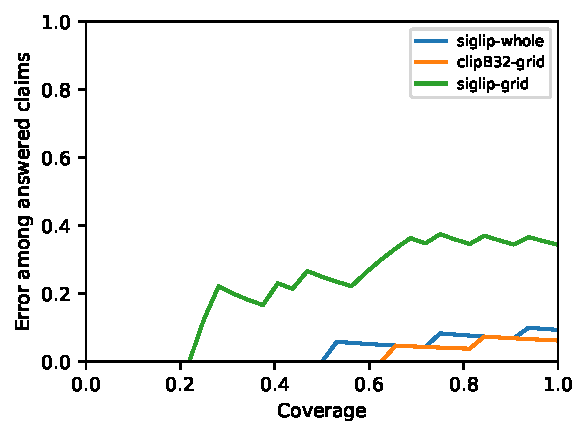
\includegraphics[width=.49\columnwidth]{risk_coverage.pdf}
\caption{Raw-score reliability and risk--coverage on the common exploratory
cohort. Scores are not calibrated probabilities. Curves do not imply a formal
risk guarantee or a threshold selected on an isolated calibration set.}
\label{fig:cal}
\end{figure}
Matched-cohort ECE is 0.2585, 0.2966 and 0.3492 for whole SigLIP, CLIP-grid and
SigLIP-grid. These scores should not be presented as calibrated probabilities.
The supplied logistic calibration routine fits only an explicit calibration
partition and rejects overlapping evaluation groups. Calibrated test results
and formal high-confidence risk guarantees are \missing. Reliability and
risk--coverage curves in Fig.~\ref{fig:cal} describe raw archived scores only.

\section{Efficiency, Ablation, and Failure Analysis}
Real API smoke traces now record prompts, returned model versions, tokens,
service times and stage outcomes on one existing development image. One input
is a generated answer; another is an author-edited derivative. These are
functional smoke tests, not independently adjudicated repair experiments.
Shared replay calls are separated from real network calls. Old aggregate
timings mix downloads, loading and multiple methods; they cannot establish
per-model latency or cost savings. GPU latency, peak RAM, API prices and cost
per thousand examples remain \missing.

Full-component ablations, authentic external baselines, natural diagnosis
accuracy, cross-model/dataset transfer and independently judged answer
preservation are \missing. A queue of 67 legacy examples is supplied for
blinded review; no fifty-case manual annotation claim is made. Failure classes
include false positives/negatives, wrong routing, failed repair,
overcorrection, verifier failure and visually ambiguous evidence.

For future repair evaluation, report corrected hallucinated answers $F$,
originally correct answers lost $B$, and utility $(F-B)/N$, alongside final
answer correctness and hallucination reduction. Abstention is not counted in
$F$; removal of a correct answer contributes to $B$. This prevents an
abstain-everything policy from appearing to repair every error.

\section{Discussion, Limitations, and Ethics}
Claim granularity can expose local failures, but decomposition and verifier
errors propagate. Multiple channels may complement one another without being
independent. A useful diagnosis must predict intervention outcomes beyond
what a scalar detector or direct outcome policy predicts. That hypothesis
remains unresolved. CPU-local models enable accessible deployment; API calls
shift compute remotely and introduce cost, privacy and version dependence.

Limitations include development reuse, small clustered cohorts, synthetic
training, unvalidated causal categories, semantic/negation ambiguity, detector
duplicate boxes, difficult OCR/relations, unknown pretraining contamination
and missing independent repair labels. Dataset rights must be checked per
source/image. Uploaded images should be sent remotely only with user consent.
Human judges must remain distinct from the model used to approve repairs.

\section{Conclusion}
V-TRACE+ currently demonstrates inspectable compatibility scoring and an
executable diagnosis--route--repair--verify protocol, not validated superior
mitigation. Matched-coverage analysis removes an earlier claimed selective
advantage, and synthetic shift exposes diagnosis shortcuts. The next scientific
milestone is a sealed, independently annotated preservation-and-cost comparison
against fixed and outcome-based repair policies. Auditing these weaknesses is
more informative than adding unvalidated model components.

\section*{Evidence and Reproduction}
All paper numbers derive from \texttt{results/audited/report.json} and
\texttt{synthetic\_gbm.json}; source hashes and input cohorts are recorded.
\texttt{research.analyze}, \texttt{research.synthetic\_diagnosis} and
\texttt{research.report\_assets} reproduce tables/figures. API traces are in
\texttt{experiments/}; gold remains absent. Full numerical provenance and
unsupported claims are documented in \texttt{claim\_audit.md}.

\begin{thebibliography}{99}
\bibitem{chair} A. Rohrbach et al., ``Object hallucination in image captioning,'' EMNLP, 2018.
\bibitem{pope} Y. Li et al., ``Evaluating object hallucination in large vision-language models,'' EMNLP, 2023, arXiv:2305.10355.
\bibitem{amber} J. Wang et al., ``AMBER: An LLM-free multi-dimensional benchmark for MLLMs hallucination evaluation,'' arXiv:2311.07397, 2023.
\bibitem{hallusion} T. Guan et al., ``HallusionBench: An advanced diagnostic suite for entangled language hallucination and visual illusion in large vision-language models,'' CVPR, 2024.
\bibitem{rlhf} Z. Sun et al., ``Aligning large multimodal models with factually augmented RLHF,'' arXiv:2309.14525, 2023.
\bibitem{mhal} A. Gunjal, J. Yin, and E. Bas, ``Detecting and preventing hallucinations in large vision language models,'' AAAI, 2024.
\bibitem{faith} L. Jing, R. Li, Y. Chen, and X. Du, ``FaithScore: Fine-grained evaluations of hallucinations in large vision-language models,'' Findings of EMNLP, 2024.
\bibitem{wood} S. Yin et al., ``Woodpecker: Hallucination correction for multimodal large language models,'' Science China Information Sciences, 2024, arXiv:2310.16045.
\bibitem{vcd} S. Leng et al., ``Mitigating object hallucinations in large vision-language models through visual contrastive decoding,'' CVPR, 2024.
\bibitem{opera} Q. Huang et al., ``OPERA: Alleviating hallucination in multi-modal large language models via over-trust penalty and retrospection-allocation,'' CVPR, 2024.
\bibitem{halc} Z. Chen et al., ``HALC: Object hallucination reduction via adaptive focal-contrast decoding,'' ICML, 2024.
\bibitem{m3id} A. Favero et al., ``Multi-modal hallucination control by visual information grounding,'' CVPR, 2024, arXiv:2403.14003.
\bibitem{selective} Y. Geifman and R. El-Yaniv, ``Selective classification for deep neural networks,'' arXiv:1705.08500, 2017.
\bibitem{calibration} C. Guo et al., ``On calibration of modern neural networks,'' ICML, 2017.
\bibitem{selfcheck} P. Manakul, A. Liusie, and M. J. F. Gales, ``SelfCheckGPT: Zero-resource black-box hallucination detection for generative large language models,'' EMNLP, 2023.
\bibitem{route} I. Ong et al., ``RouteLLM: Learning to route LLMs with preference data,'' arXiv:2406.18665, 2024.
\bibitem{visor} Y. Zhang, C. Zhan, and H. Wang, ``When visual signals mislead: A mechanistic study of attribute hallucination in vision-language models,'' arXiv:2608.11024, 2026.
\bibitem{safe} M. Fazli et al., ``Does playing it safe count as faithfulness? Reassessing LVLM hallucination mitigation methods,'' arXiv:2609.01888, 2026.
\end{thebibliography}
\end{document}
